%!TEX root = ../report.tex
\chapter{ROS Nodes Structure} % (fold)
\label{chap:ros_nodes_structure}
The ROS nodes structure implemented and its topics are showed in Figure \ref{fig:ros_nodes} and introduced below:
\begin{enumerate}
	\item \textbf{Ball tracker}. This node receives images from the stereo rig in compressed format, extracts the 2D position of the marker in both images and reconstructs its position in the 3D space. 
	The coordinates of the point are then published. The algorithm encoded within this node is broken down in chapters [\ref{chap:feature_extraction}] and [\ref{chap:stereopsis}].
	\item \textbf{Kalman filter}. The input new point is used here to predict the future state based on the physical model. This node lets the robot keep moving even when the cameras have lost the target. 
	A detailed explanation of the node tasks can be found in chapter [\ref{chap:prediction}].
	\item \textbf{Path planning}. Once the point has been located in the three-dimensional space, a new joint configuration subject to some constraints is calculated in order to keep the object tracking the target. 
	The path planning node is explained in chapter [\ref{chap:path_planning}].
	\item \textbf{Points server}. An auxiliary node has been developed for providing virtual points to the system in a modular fashion. 
	It has been employed to perform the simulations prior the use of the workcell.
	\item \textbf{RobWork Studio plugin}. To improve the visioning of the robot and its movements, a real-time viewer plugin has been developed for RobWorkStudio. 
	This plugin enables the real time simulation of the input 3D points in the system and has helped testing the algorithm performance off line.
	\item \textbf{Log}. A new log node has been implemented for our task. 
	This node subscribes to all the relevant topics in the structure and generates in real time the graphics used for the analysis of the system.
\end{enumerate}

\begin{figure}[!ht]
	\centering
	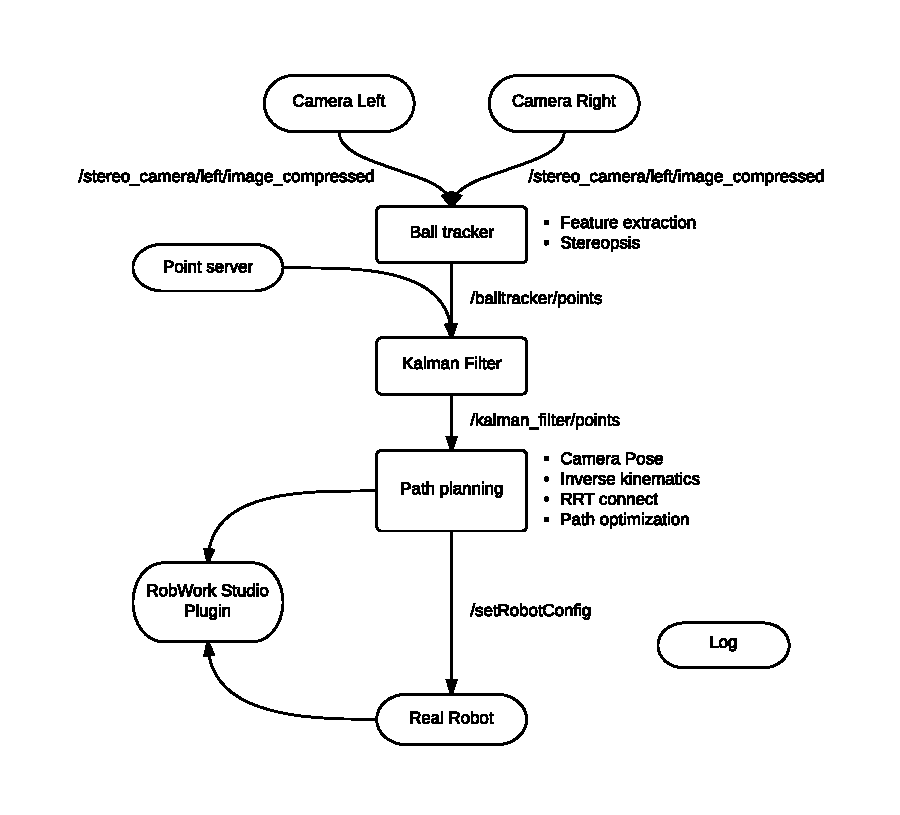
\includegraphics[width=\textwidth]{figures/ros_nodes}
	\caption{ROS Nodes implemented}
	\label{fig:ros_nodes}
\end{figure}
% chapter ros_nodes_structure (end)